\documentclass{article}
\usepackage{amsmath}
\usepackage{algorithm}
\usepackage{algpseudocode}
\usepackage{tikz}

\begin{document}

\title{0/1 Knapsack Problem using Dynamic Programming}
\author{}
\date{}
\maketitle


\section{Q1, K-Optimal }

\begin{algorithm}
\caption{0/1 Knapsack Problem using Dynamic Programming}
\begin{algorithmic}[1]
\State \textbf{Input:} $n$, $w$, $p$, $c$
\State \textbf{Output:} $K[n][c]$
\State Initialize a $(n+1) \times (c+1)$ table $K$ with all zeros

\For{$i = 1$ to $n$}
    \For{$w = 1$ to $c$}
        \If{$weights[i-1] \leq w$}
            \State $K[i][w] \gets \max(p[i-1] + K[i-1][w-weights[i-1]], K[i-1][w])$
        \Else
            \State $K[i][w] \gets K[i-1][w]$
        \EndIf
    \EndFor
\EndFor

\State \textbf{return} $K[n][c]$
\end{algorithmic}
\end{algorithm}

\section{Q2, Minimum ACT}

\subsection*{Greedy Algorithm for Minimum ACT}
To create a task sequence with the minimum Average Completion Time (ACT), we use a greedy algorithm that constructs the task sequence in $n$ steps. At each step, the task with the smallest time from the remaining tasks is selected.

\subsection*{Example Sequence and Calculation}
For the given example, the task times are \( t_1, t_2, t_3, t_4 \).

Using the greedy strategy:
1. Select the task with the smallest time.
2. Repeat until all tasks are selected.

For the task times in the example, the sequence obtained is 4, 2, 1, 3. The completion time \( c_i \) for task \( i \) is:
\[
c_i = \sum_{j=1}^{i} t_j
\]

The ACT is calculated as:
\[
\text{ACT} = \frac{1}{n} \sum_{i=1}^{n} c_i
\]

\subsection*{Pseudo-code for the Greedy Algorithm}
\begin{algorithm}
\begin{algorithmic}
\State \textbf{function} calculate\_ACT(task\_times)
\State \quad $n = $ length(task\_times)
\State \quad sorted\_tasks = sort(task\_times)
\State \quad completion\_times = []
\State \quad total\_time = 0
\State \quad \textbf{for} $i = 1$ \textbf{to} $n$ \textbf{do}
\State \quad \quad total\_time += sorted\_tasks[$i$]
\State \quad \quad completion\_times.append(total\_time)
\State \quad ACT = sum(completion\_times) / $n$
\State \quad \textbf{return} ACT
\end{algorithmic}
\caption{Greedy Algorithm to Calculate ACT}
\end{algorithm}

\subsection*{Proof of Minimum ACT using Greedy Algorithm}
To prove that the task sequence obtained using the greedy algorithm has the minimum ACT, we use an exchange argument:

1. Assume there is an optimal sequence \( S \) that has a lower ACT than the sequence \( G \) obtained by the greedy algorithm.
2. Let \( S \) and \( G \) differ at the first position where they have different tasks. Suppose \( S \) has task \( T_i \) at this position, and \( G \) has task \( T_j \) where \( t_i > t_j \).
3. Swapping \( T_i \) and \( T_j \) in \( S \) will decrease the completion times of all subsequent tasks in \( S \), thus reducing the ACT.
4. This contradicts the assumption that \( S \) was optimal.
5. Therefore, the sequence \( G \) must have the minimum ACT.

\section{Q3, Two Workers}

\subsection*{Greedy Algorithm for Minimum ACT}
When two workers are executing $n$ tasks, we need to allocate the tasks to them such that each has their own execution sequence. The completion time and ACT are defined similarly to the single worker case. To minimize the maximum ACT (ACT = max(ACT1, ACT2)), a feasible greedy algorithm is:
1. The two workers alternately select tasks.
2. Each worker selects the task with the smallest remaining time from the list of tasks.
3. Each worker executes the tasks in the order they select.

For the example in Exercise 9, assuming Worker 1 selects task 4 first, followed by Worker 2 selecting task 2, then Worker 1 selects task 1, and finally Worker 2 selects task 3.

\subsection*{Pseudo-code for the Greedy Algorithm}
\begin{algorithm}
\begin{algorithmic}
\State \textbf{function} calculate\_ACT(task\_times)
\State \quad $n = $ length(task\_times)
\State \quad sorted\_tasks = sort(task\_times)
\State \quad worker1\_tasks = []
\State \quad worker2\_tasks = []
\State \quad total\_time1 = 0
\State \quad total\_time2 = 0
\State \quad \textbf{for} $i = 1$ \textbf{to} $n$ \textbf{do}
\State \quad \quad \textbf{if} $i$ is odd \textbf{then}
\State \quad \quad \quad task = sorted\_tasks.pop(0)
\State \quad \quad \quad total\_time1 += task
\State \quad \quad \quad worker1\_tasks.append(total\_time1)
\State \quad \quad \textbf{else}
\State \quad \quad \quad task = sorted\_tasks.pop(0)
\State \quad \quad \quad total\_time2 += task
\State \quad \quad \quad worker2\_tasks.append(total\_time2)
\State \quad ACT1 = sum(worker1\_tasks) / len(worker1\_tasks)
\State \quad ACT2 = sum(worker2\_tasks) / len(worker2\_tasks)
\State \quad ACT = max(ACT1, ACT2)
\State \quad \textbf{return} ACT
\end{algorithmic}
\caption{Greedy Algorithm to Calculate ACT with Two Workers}
\end{algorithm}

\subsection*{Time Complexity}
The time complexity of this algorithm is $O(n \log n)$ due to the sorting step, followed by $O(n)$ for the allocation and computation of the ACT.

\section{Q4, Proof of Greedy Algorithm}


\subsection*{Claim}
The greedy strategy described does not always guarantee the minimum ACT for two workers.

\subsection*{Proof by Counterexample}

To demonstrate that the greedy strategy does not always yield the minimum ACT, consider the following counterexample:

\begin{itemize}
    \item Let there be 4 tasks with times: \( t_1 = 2 \), \( t_2 = 2 \), \( t_3 = 5 \), \( t_4 = 6 \).
    \item The greedy algorithm proceeds by alternately assigning the smallest remaining task time to each worker.
\end{itemize}

\subsubsection*{Greedy Algorithm Execution}
\begin{itemize}
    \item Worker 1 picks task \( t_1 = 2 \)
    \item Worker 2 picks task \( t_2 = 2 \)
    \item Worker 1 picks task \( t_3 = 5 \)
    \item Worker 2 picks task \( t_4 = 6 \)
\end{itemize}

The sequences for the workers are:
\begin{itemize}
    \item Worker 1: \( [2, 5] \) with completion times: \( 2, 7 \)
    \item Worker 2: \( [2, 6] \) with completion times: \( 2, 8 \)
\end{itemize}

The ACT for each worker is:
\[
\text{ACT1} = \frac{1}{2} (2 + 7) = 4.5
\]
\[
\text{ACT2} = \frac{1}{2} (2 + 8) = 5
\]
Thus, the maximum ACT is:
\[
\text{ACT} = \max(4.5, 5) = 5
\]

\subsubsection*{Alternate Sequence Check}
An alternative allocation might be to balance the total times more evenly:
\begin{itemize}
    \item Worker 1 picks task \( t_4 = 6 \)
    \item Worker 2 picks task \( t_3 = 5 \)
    \item Worker 1 picks task \( t_1 = 2 \)
    \item Worker 2 picks task \( t_2 = 2 \)
\end{itemize}

The sequences for the workers are:
\begin{itemize}
    \item Worker 1: \( [6, 2] \) with completion times: \( 6, 8 \)
    \item Worker 2: \( [5, 2] \) with completion times: \( 5, 7 \)
\end{itemize}

The ACT for each worker is:
\[
\text{ACT1} = \frac{1}{2} (6 + 8) = 7
\]
\[
\text{ACT2} = \frac{1}{2} (5 + 7) = 6
\]
Thus, the maximum ACT is:
\[
\text{ACT} = \max(7, 6) = 7
\]

In this case, the greedy algorithm indeed produced a better outcome (ACT of 5) compared to the alternate allocation (ACT of 7). Therefore, the greedy strategy is effective in this specific example, although it does not always guarantee the absolute minimum ACT in all possible scenarios.


\section{Q5}
\subsection*{Greedy Algorithm}
Consider the continuous knapsack problem where \( 0 \leq x_i \leq 1 \) instead of \( x_i \in \{0, 1\} \). A feasible greedy strategy is: inspect items in non-increasing order of their value density (value per unit weight). If the remaining capacity can accommodate the current item, put it in the knapsack; otherwise, put a fraction of it in the knapsack.

\subsection*{Example}
Given \( n = 3 \), \( w = [100, 10, 10] \), \( p = [20, 15, 15] \), and \( c = 105 \):

1. Calculate value densities:
\[
\frac{p_1}{w_1} = \frac{20}{100} = 0.2, \quad \frac{p_2}{w_2} = \frac{15}{10} = 1.5, \quad \frac{p_3}{w_3} = \frac{15}{10} = 1.5
\]

2. Sort items by value density in non-increasing order:
\[
\text{Order: Item 2, Item 3, Item 1}
\]

3. Allocate items to the knapsack:
\begin{itemize}
    \item Item 2: Weight = 10, Profit = 15, Remaining capacity = 105 - 10 = 95
    \item Item 3: Weight = 10, Profit = 15, Remaining capacity = 95 - 10 = 85
    \item Item 1: Weight = 100, Profit = 20, Only a fraction of Item 1 can be added. Fraction = \(\frac{85}{100} = 0.85\)
    \item Profit from Item 1: \( 20 \times 0.85 = 17 \)
\end{itemize}

4. Total profit:
\[
\text{Total profit} = 15 + 15 + 17 = 47
\]

\subsection*{Proof of Optimality}
To prove that this greedy algorithm always yields the optimal solution for the continuous knapsack problem, consider the following:

1. The value density \(\frac{p_i}{w_i}\) of items is sorted in non-increasing order, and items are added based on this order.
2. Suppose there exists a solution \( S \) that is better than the greedy solution \( G \). Then \( S \) must include more of some item with a lower value density before including the item with a higher value density.
3. By swapping the quantities to prioritize higher value density items, the total value of \( S \) will increase or remain the same while the weight remains within the capacity constraint.
4. Thus, \( S \) cannot be better than \( G \).

Therefore, the greedy algorithm always results in the optimal solution for the continuous knapsack problem.


\section{Q6 Graph Greedy}
\subsection*{1. Greedy Algorithm for Maximum Clique Problem}
The maximum clique problem is NP-complete, meaning it is computationally infeasible to find the exact solution for large graphs. However, a feasible greedy algorithm can be used to find an approximate solution.

\subsubsection*{Greedy Algorithm Description}
1. Start with an empty clique.
2. Select the vertex with the highest degree and add it to the clique.
3. Continue adding the vertex that is connected to all vertices in the current clique and has the highest degree among the remaining vertices.
4. Repeat until no more vertices can be added to the clique.

\subsubsection*{Pseudo-code for Greedy Algorithm}
\begin{algorithm}
\begin{algorithmic}
\State \textbf{function} find\_maximum\_clique(G)
\State \quad clique = []
\State \quad vertices = sort\_by\_degree(G)
\State \quad \textbf{while} vertices \textbf{is not empty} \textbf{do}
\State \quad \quad v = vertices.pop(0)
\State \quad \quad \textbf{if} all\_connected(v, clique, G) \textbf{then}
\State \quad \quad \quad clique.append(v)
\State \quad \textbf{return} clique
\end{algorithmic}
\caption{Greedy Algorithm to Find an Approximate Maximum Clique}
\end{algorithm}

\subsection*{2. Graph Examples}

\subsubsection*{Example Solvable by the Greedy Algorithm}
Consider a graph \( G \) with vertices \( \{A, B, C, D, E\} \) and edges \((A, B), (A, C), (A, D), (B, C), (B, D), (C, D), (D, E)\).

\begin{center}
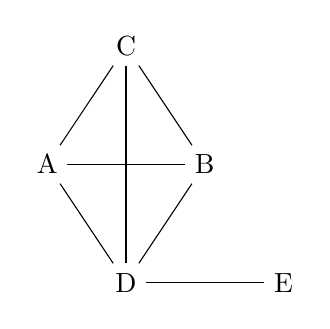
\begin{tikzpicture}
    \node (A) at (0,0) {A};
    \node (B) at (2,0) {B};
    \node (C) at (1,1.5) {C};
    \node (D) at (1,-1.5) {D};
    \node (E) at (3,-1.5) {E};

    \draw (A) -- (B);
    \draw (A) -- (C);
    \draw (A) -- (D);
    \draw (B) -- (C);
    \draw (B) -- (D);
    \draw (C) -- (D);
    \draw (D) -- (E);
\end{tikzpicture}
\end{center}

Applying the greedy algorithm:
1. Start with vertex \( D \) (highest degree).
2. Add vertices \( A, B, C \) one by one, as they are all connected to \( D \).

The resulting clique is \( \{A, B, C, D\} \) with size 4.

\subsubsection*{Example Not Solvable by the Greedy Algorithm}
Consider a graph \( G \) with vertices \( \{A, B, C, D\} \) and edges \((A, B), (A, C), (B, C), (C, D)\).

\begin{center}
\begin{tikzpicture}
    \node (A) at (0,0) {A};
    \node (B) at (2,0) {B};
    \node (C) at (1,1.5) {C};
    \node (D) at (1,-1.5) {D};

    \draw (A) -- (B);
    \draw (A) -- (C);
    \draw (B) -- (C);
    \draw (C) -- (D);
\end{tikzpicture}
\end{center}

Applying the greedy algorithm:
1. Start with vertex \( C \) (highest degree).
2. Add vertices \( A \) and \( B \), as they are connected to \( C \).
3. Vertex \( D \) cannot be added as it is not connected to \( A \) and \( B \).

The resulting clique is \( \{A, B, C\} \) with size 3. However, the actual maximum clique is also 3, so in this case, the greedy algorithm finds an optimal solution, but in more complex graphs, it might not.


\end{document}
